\newcommand{\xs}{4.5 cm}
\newcommand{\totscale}{.6}
\newcommand{\afmscale}{.42}
\begin{tikzpicture}[scale=\totscale]
	%SB02-3
	\begin{scope}[xshift=\xs]
		\node at (0,0) {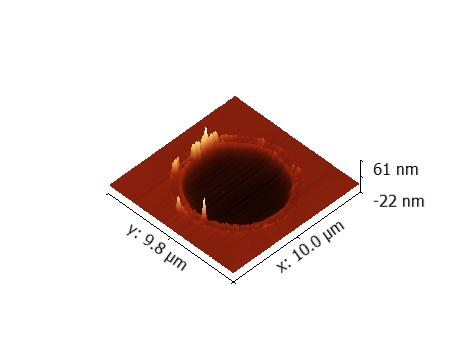
\includegraphics[scale=\afmscale]{Figs_Friction/AFM_SB02-3.jpg}};
		\node at (0,-4.5 cm) {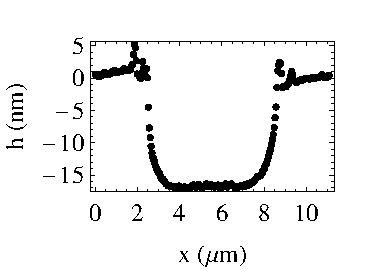
\includegraphics[scale=\totscale]{Figs_Friction/Section_SB02-3.pdf}};
		\node at (0,-10 cm) {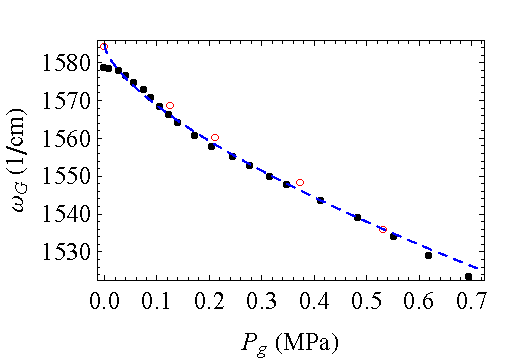
\includegraphics[scale=\totscale]{Figs_Friction/CenterFit_SB02-3.pdf}};
	\end{scope}
	%SB03-2b
	\begin{scope}[xshift=-\xs]
		\node at (0,0) {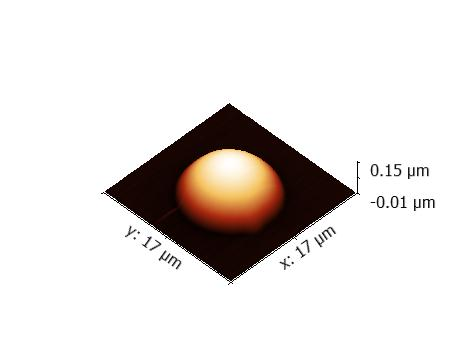
\includegraphics[scale=\afmscale]{Figs_Friction/AFM_SB03-2A.jpg}};
		\node at (0,-4.5 cm) {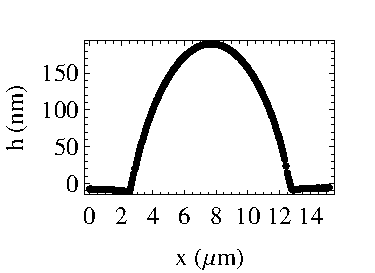
\includegraphics[scale=\totscale]{Figs_Friction/Section_SB03-2A.pdf}};
		\node at (0,-10 cm) {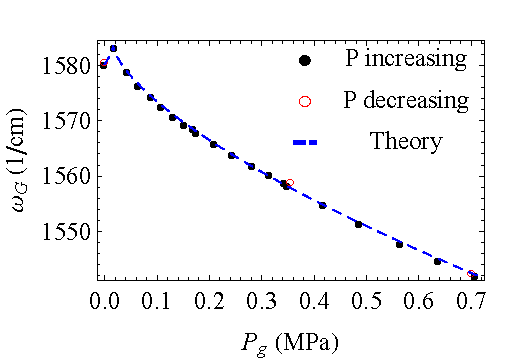
\includegraphics[scale=\totscale]{Figs_Friction/CenterFit_SB03-2A.pdf}};
	\end{scope}
	
	\node at (.7,1.75) [anchor=south west]{\textbf{(b)}  Snapped to side wall};
	\node at (-8,1.75) [anchor=south west]{\textbf{(a)} $P_0>P_a$};
\end{tikzpicture}